
\FloatBarrier
\section{Колебательная система с гистерезисом в возвращающей силе} %  % {{{1 _VGLASS_
\label{atu:sect:vglass}

\LinkRef{
  vglass: ITMM-2013
}

\subsection{Определение системы и анализ её динамики} %  % {{{2 _vglass_task

Колебательные системы с различными видами нелинейностями
как в возвращающей силе, так и члене при первой производной,
часто рассматриваются как потенциальные кандидаты в хаотические системы.
Особый интерес представляют системы, нелинейные компоненты которых
отображают реальные элементы систем управления~\cite{atu_st85,atu_ISDMCI2013,atu_asau20}.
Одним из таких существенно нелинейных элементов
является гистерезис~\cite{sys_hyst,in_theory_mech_vibro,ivanov_alg_id_dyn_hyst,andronn_id_ns_hyst,mai_iss_dyn_isp}.
Рассмотрим изначально неустойчивую  систему,
которая стабилизируется релейно-пропорциональным
стабилизирующим воздействием.
Такая система стабилизации активируется при заданном отклонении наблюдаемой
величины, а выключается при меньшем. Такая неоднозначность в поведении
систем стабилизации приводит к разнообразным колебательным явлениям вблизи
точки стабилизации, а все попытки линеаризации рассматриваемых
нелинейностей, в данном случае, приводят к принципиальным ошибкам в
моделировании.

Наличие точки неустойчивого равновесия, требующего стабилизирующего
воздействия в большем масштабе, явной, а зачастую и скрытой нелинейности
элементов системы, априорная параметрическая неопределенность внешних
воздействий, --- всё это создаёт предпосылки для появления у систем сложной
колебательной динамики, в том числе и хаотической.
Рассмотрим уравнение, задающее динамику этой системы:
%
\begin{equation}
  \ddot{x} + c_o \dot{x} + r( x, \ldots ) = u(t),
  \label{atu:eq:vglass}
\end{equation}
%
где
$x(t)$ -- координата (выходной сигнал),
$ c_0$ -- безразмерный коэффициент демпфирования,
$u(t) = U_{in} \sin( \omega_{in} t ) $ -- внешняя возмущающая сила,
$r( x, \ldots) $ --- возвращающая сила,
включающая линейную составляющую ($ax$, $a<0$),
обуславливающую неустойчивость при малых отклонениях,
и гистерезисную компоненту, которая задаётся алгоритмически.
Характерный вид возвращающий силы приведён на  рис.~\ref{atu:f:vg_rf}.

\begin{figure}[htb!]
\centerline{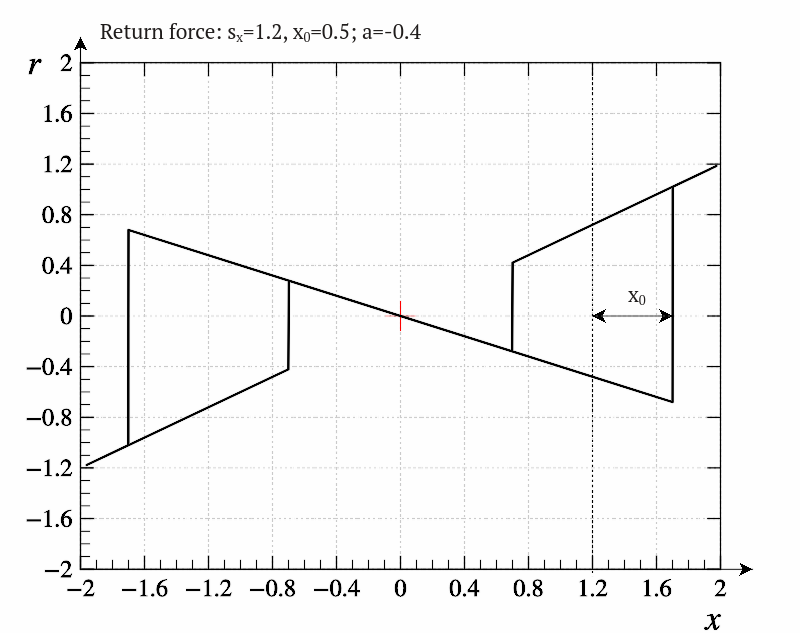
\includegraphics[width=0.5\textwidth]{p/cha/vg/vg_rf-p_rf.png} }
\caption{Гистерезисная возвращающая сила}
\label{atu:f:vg_rf}
\end{figure}

Параметрами этой зависимости, помимо уже упомянутого коэффициента $a$,
являются $s_x$ --- центральная точка включения и выключения
стабилизирующего воздействия,
$x_0$ --- полуширина гистерезиса.
Ширина петли гистерезиса для данной системы определяет
энергию, которую получает система от системы стабилизации в процессе работы.
Именно это величина и будет идентифицируемым параметром.


В отличие от системы Дуффинга, рассматриваемая система имеет собственную
динамику при отсутствии возмущающего воздействия.
При малых значениях $x_0$ происходят нелинейные,
но достаточно простые колебания по одну сторону от
точки $x=0$~(рис.~\ref{atu:f:vglass_phase_f_u00}),
причём сторона определяется начальными условиями.
Спектр колебаний весьма бедный.

\begin{figure}[ht!]
\begin{center}
  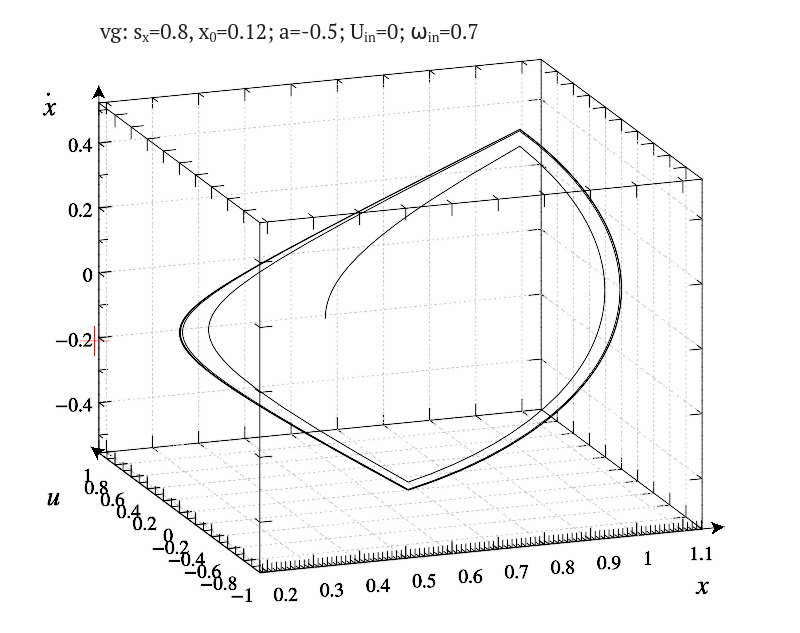
\includegraphics[width=0.49\textwidth]{p/cha/vg/vg_0-p_phe_0x00_0x70_0x12.png}
  \hfill
  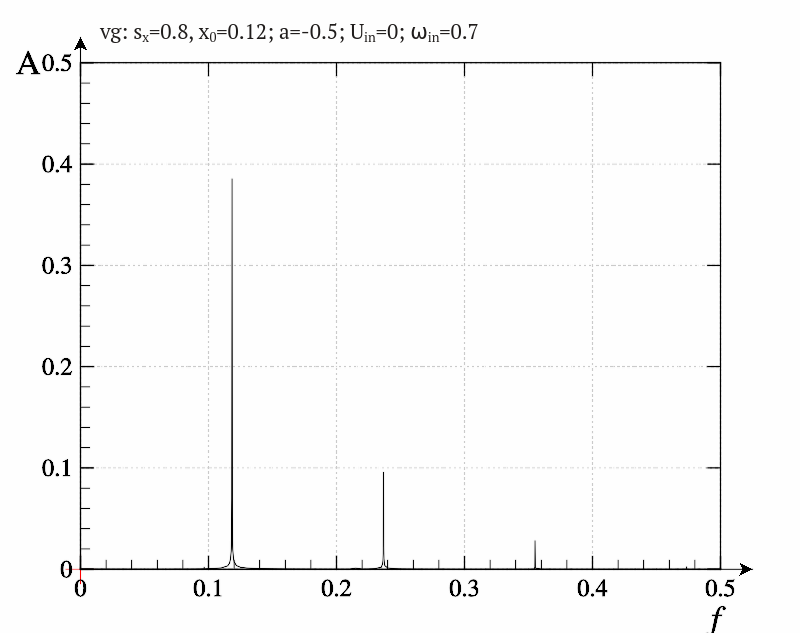
\includegraphics[width=0.49\textwidth]{p/cha/vg/vg_fft-p_f_0x00_0x70_0x12.png}
\end{center}
  \caption{Расширенный фазовый портрет и спектр системы (\ref{atu:eq:vglass}) при $U_{in}=0$ и $x_0=0.12$}
\label{atu:f:vglass_phase_f_u00}
\end{figure}

При росте параметра $x_0$ динамика системы становится более сложной
(рис.~\ref{atu:f:vglass_phase_f_u01}),
однако спектр системы остаётся простым линейчатым.
Такое поведение сохраняется вплоть до естественного ограничения $x_o < s_x$,
при этом фазовый портрет приближается к окружности.

\begin{figure}[ht!]
\begin{center}
  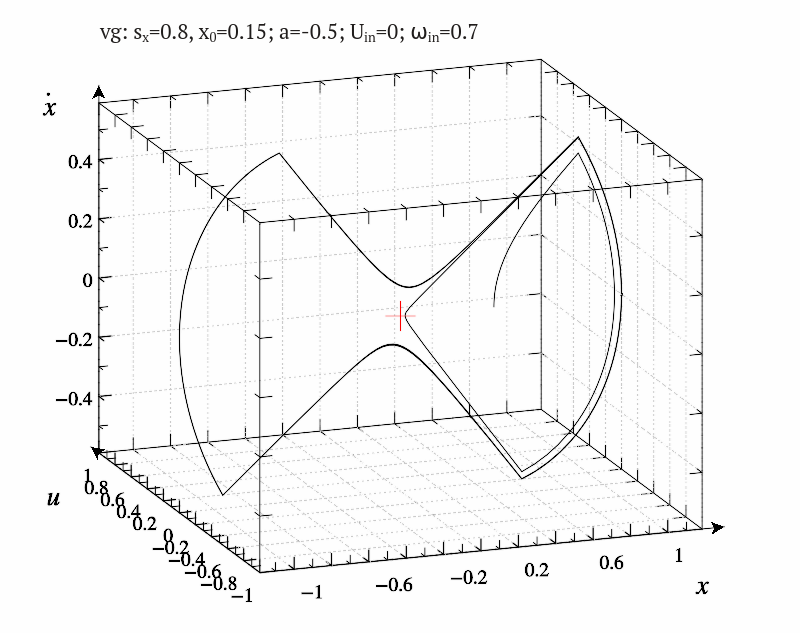
\includegraphics[width=0.49\textwidth]{p/cha/vg/vg_0-p_phe_0x00_0x70_0x15.png}
  \hfill
  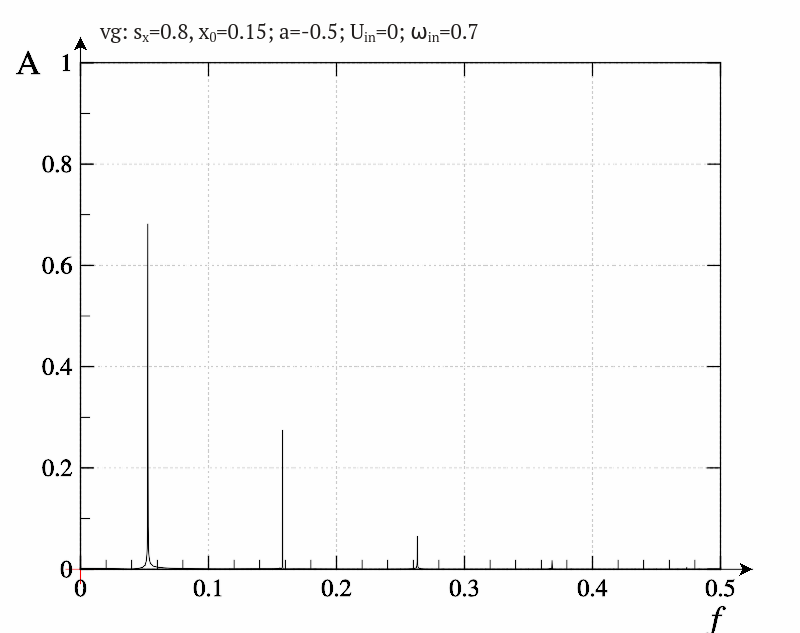
\includegraphics[width=0.49\textwidth]{p/cha/vg/vg_fft-p_f_0x00_0x70_0x15.png}
\end{center}
  \caption{Расширенный фазовый портрет и спектр системы (\ref{atu:eq:vglass}) при $U_{in}=0$ и $x_0=0.15$}
\label{atu:f:vglass_phase_f_u01}
\end{figure}

При наличии ненулевого внешнего воздействия $u(t)$
картина заметно усложняется.
Наблюдаются такие значения параметра $x_0$,
при которых наблюдается сложный аттрактор, характерный для
хаотической динамики~(рис.~\ref{atu:f:vglass_phase_f_u10})
и участки сплошного спектра.

\begin{figure}[ht!]
\begin{center}
  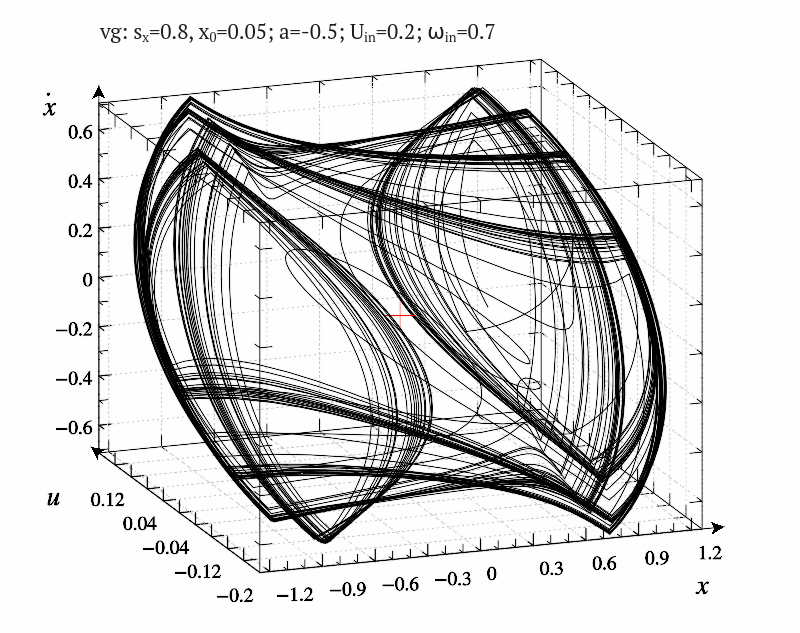
\includegraphics[width=0.49\textwidth]{p/cha/vg/vg_0-p_phe_0x20_0x70_0x05.png}
  \hfill
  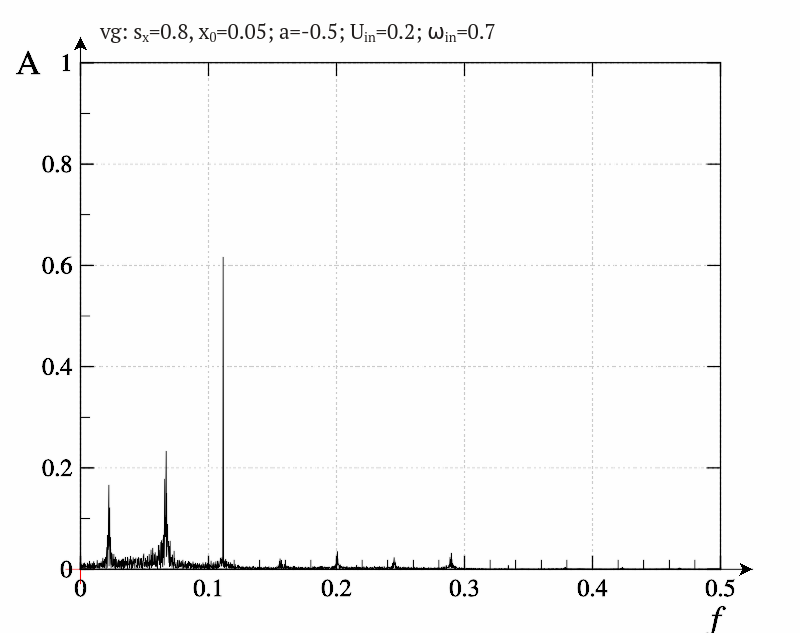
\includegraphics[width=0.49\textwidth]{p/cha/vg/vg_fft-p_f_0x20_0x70_0x05.png}
\end{center}
  \caption{Расширенный фазовый портрет и спектр системы (\ref{atu:eq:vglass}) при $U_{in}=0.2$ и $x_0=0.05$}
\label{atu:f:vglass_phase_f_u10}
\end{figure}

Общим свойством этой системы и системы Дуффинга является то,
что участок сплошного спектра примыкает к точке нулевой частоты,
что затрудняет процесс усреднения критерия.

Также наблюдаются такие диапазоны $x_0$,
в которых наблюдаются регулярные колебания
(рис.~\ref{atu:f:vglass_phase_f_u11}).

\begin{figure}[ht!]
\begin{center}
  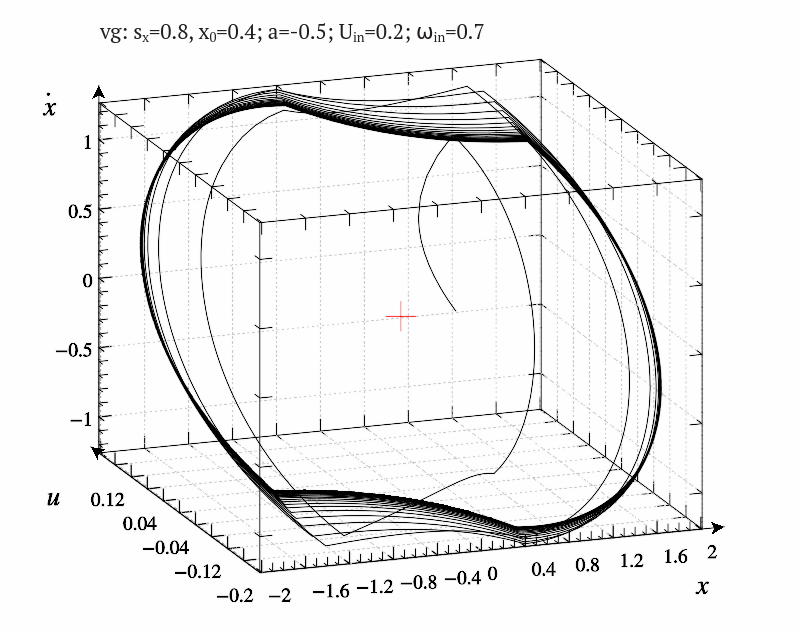
\includegraphics[width=0.49\textwidth]{p/cha/vg/vg_0-p_phe_0x20_0x70_0x40.png}
  \hfill
  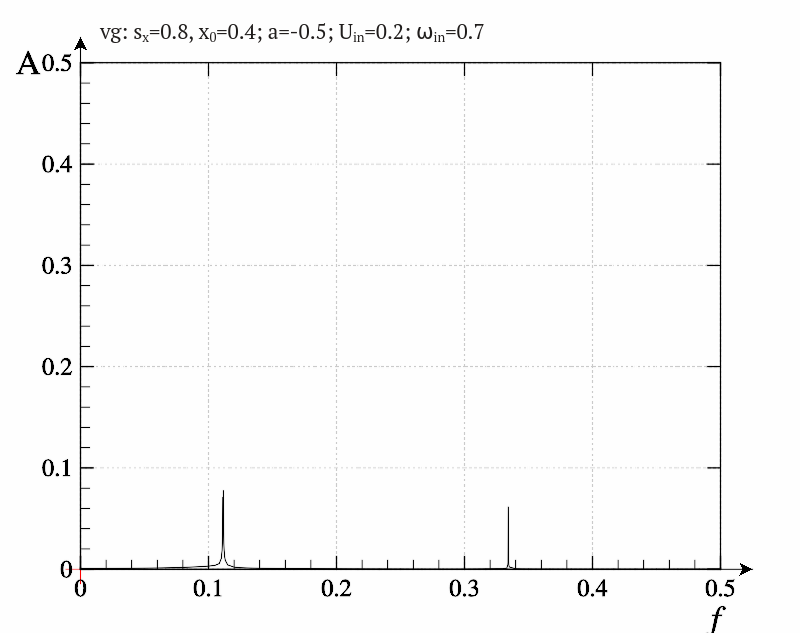
\includegraphics[width=0.49\textwidth]{p/cha/vg/vg_fft-p_f_0x20_0x70_0x40.png}
\end{center}
  \caption{Расширенный фазовый портрет и спектр системы (\ref{atu:eq:vglass}) при $U_{in}=0.2$ и $x_0=0.40$}
\label{atu:f:vglass_phase_f_u11}
\end{figure}

Помимо регулярных колебаний, наблюдаются
режимы сложно-периодической динамики,
с сложным аттрактором и спектром,
в котором наблюдаются ряд близко расположенных пиков
(рис.~\ref{atu:f:vglass_phase_f_u12}).

\begin{figure}[ht!]
\begin{center}
  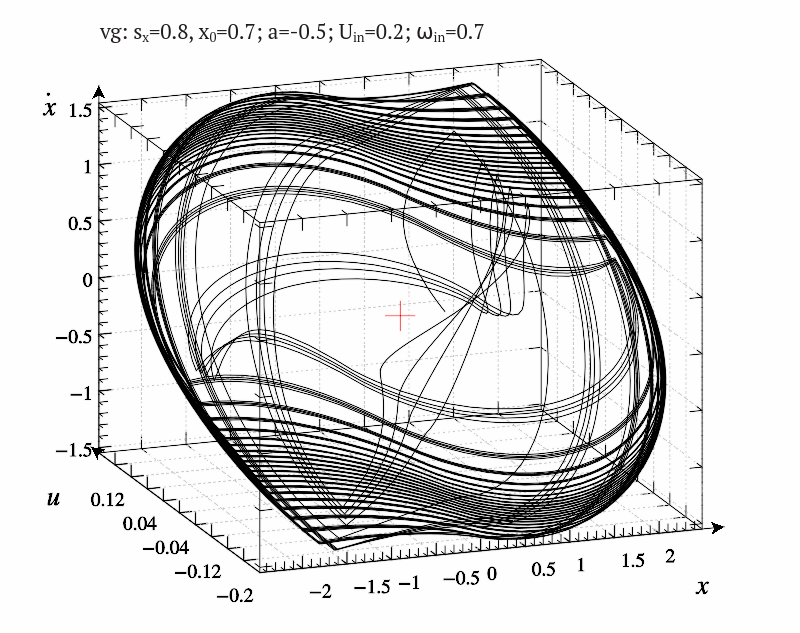
\includegraphics[width=0.49\textwidth]{p/cha/vg/vg_0-p_phe_0x20_0x70_0x70.png}
  \hfill
  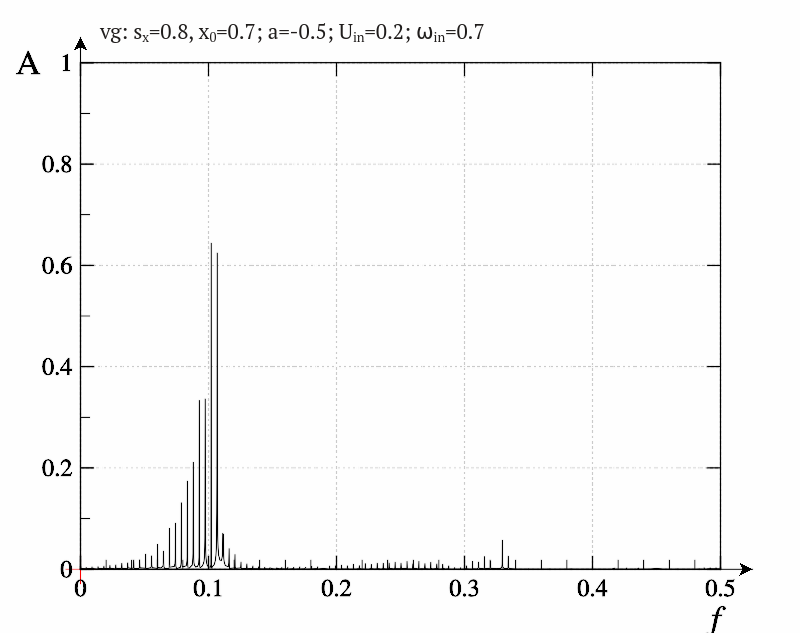
\includegraphics[width=0.49\textwidth]{p/cha/vg/vg_fft-p_f_0x20_0x70_0x70.png}
\end{center}
  \caption{Расширенный фазовый портрет и спектр системы (\ref{atu:eq:vglass}) при $U_{in}=0.2$ и $x_0=0.70$}
\label{atu:f:vglass_phase_f_u12}
\end{figure}

Такое поведение сложно, а в случае нестационарного значения параметра
может быть и невозможно отличить от хаотического поведения.

Таким образом, так как система в рабочем диапазоне параметра
$x_0$ демонстрирует различные виды динамик, в том числе хаотическую,
то для идентификации имеет смысл рассмотреть набор методов,
рассматриваемых в данной работе.

% }}}2

\subsection{Анализ и выбор критерия}  % {{{2

При синтезе критерия для нелинейной колебательной системы,
если нет возможности использовать
какой-либо явный и очевидный критерий,
в первую очередь следует рассмотреть
критерии вида $q_{x^2}$, $q_{rx}$ и $q_T$.
Так как гистерезисная возвращающая сила
не даёт возможности использовать аналитический
подход, то рассмотрим
зависимости $q_{rx}$ и $q_T$
(рис.~\ref{atu:f:vglass_q}),
полученные путём численного моделирования.

\begin{figure}[ht!]
\begin{center}
  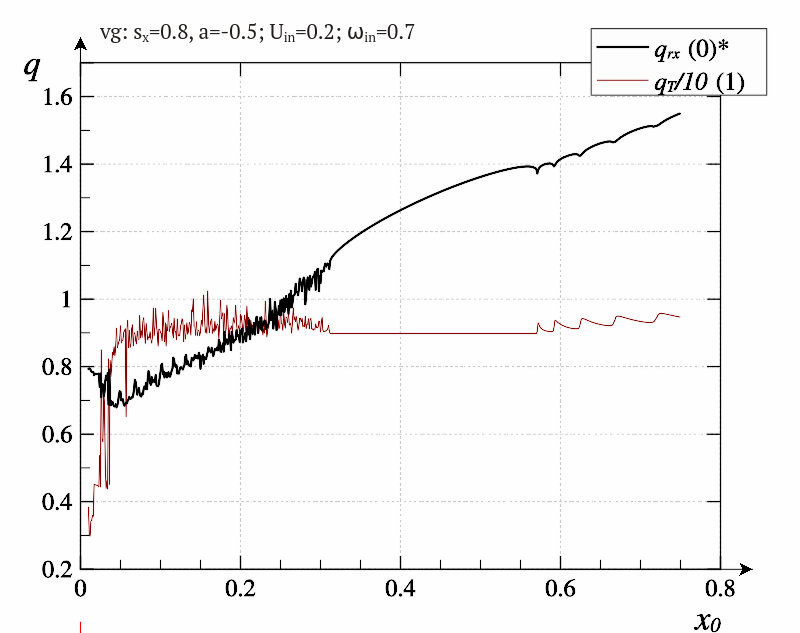
\includegraphics[width=0.49\textwidth]{p/cha/vg/vg_q1-p_q.png}
\end{center}
  \caption{Зависимости $q_{rx}(x_0)$ и $q_T(x_0)$ для системы (\ref{atu:eq:vglass})}
\label{atu:f:vglass_q}
\end{figure}

Анализ зависимостей позволяет сделать вывод о том, что критерий $q_T$
не пригоден для идентификации параметра $x_0$
рассматриваемой системы, ввиду того,
что зависимости от параметра, если не принимать во внимание колебания,
практически отсутствует.

Применений критерия $q_{rx}$ достаточно противоречиво.
С одной стороны, в целом наблюдается близкая к линейной зависимость,
что снижает требования к тонкой настройке системы идентификации.
С другой стороны, на тех участках,
где наблюдаются переходы от сложно-периодических колебаний
к хаотическим, монотонность зависимости нарушается.
Однако, амплитуда этих возмущений невелика,
что даёт возможность построения работоспособной системы идентификации,
но с существенными ограничениями на достижимую точность.
Таким образом, на неимением лучшего, будем использовать этот критерий.



% }}}2

\subsection{Тестовая задача идентификации}  % {{{2

Для идентификации параметра $x_0$
колебательной системы с гистерезисной возвращающей силой
была использована группа методов  ``ql3rlWvnAAW''.
Использование критерия $q_{rx}$ для данной системы,
с учетом наличия участков отсутствия монотонности
требует отдельной проверки работоспособности,
так как используемый ранее подход с
медленно изменяющимся параметром (\ref{atu:eq:po_t_ramp}) не позволяет
отделить ошибку, связанную с установлением режима системы идентификации
от ошибки, вызванной не вполне адекватным критерием.

Для определения ошибки идентификации без влияния переходных процессов,
была проведена серия вычислительных экспериментов.
К каждом из них значения параметра $x_0$ было фиксировано.
Диапазон изменения этого параметра был выбран $[0.2 ; 0.6]$.
Предварительно была сделана проверка, что за полное время идентификации
$T= 1000$ все переходные процессы действительно завершились.
Зависимость полученной ошибки идентификации от значения
параметра $x_0$ для различных способов оценивания $p_\mathrm{id}$
представлена на рис.~\ref{atu:f:vg_id_scan}.

\begin{figure}[ht!]
\begin{center}
  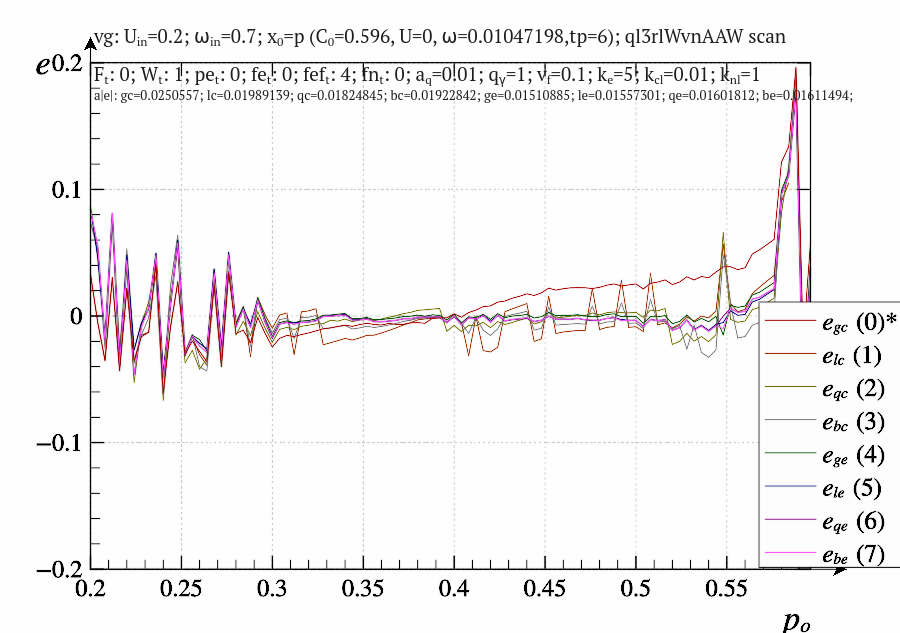
\includegraphics[width=0.60\textwidth]{p/cha/vg/vg_id-p_p_e_ql3rlWvnAAW_scan.png}
\end{center}
  \caption{Зависимости $e(x_0) $ для колебательной системы с гистерезисной возвращающей силой}
\label{atu:f:vg_id_scan}
\end{figure}

Анализ полученных зависимостей показывает, что в тех областях, где нарушается монотонность
критерия, ошибка идентификации значительно возрастает.
Однако, уровень этой ошибки, за исключением одной узкой области,
не превышает исходного расстояния между агентами,
что позволяет сделать вывод том, что система идентификации оказывается работоспособной
и этом неблагоприятном случае.

Рассмотрим динамику агентов и идентифицируемого значения (рис.~\ref{atu:f:vg_id_sign}) в случае
существенно нестационарного параметра.
При этом динамика величины $x_0(t)$ задаётся (\ref{atu:eq:po_t_sign}),
$p_0=0.4$, $U_p=0.14$, $\omega_p= 0.01048$.

\begin{figure}[ht!]
\begin{center}
  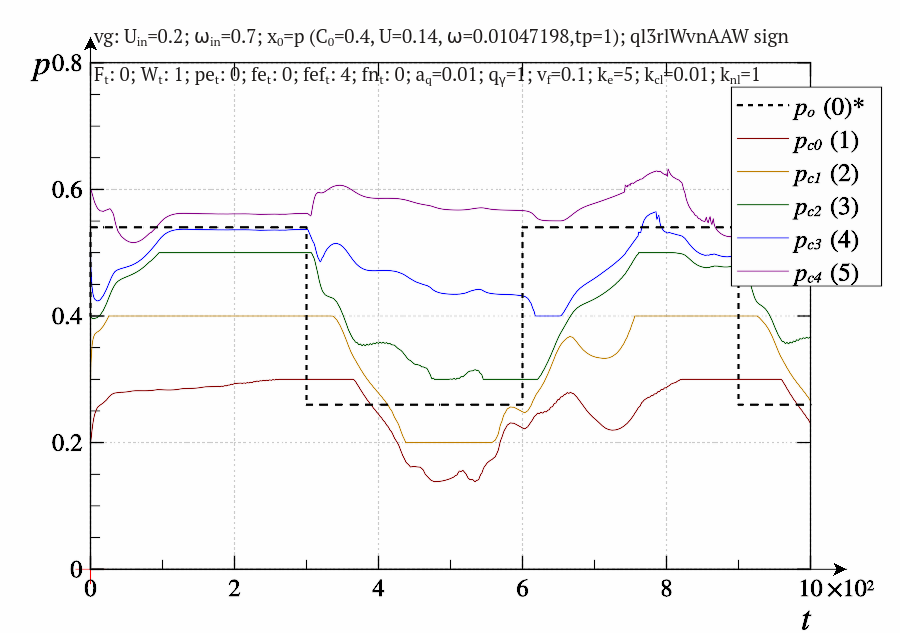
\includegraphics[width=0.49\textwidth]{p/cha/vg/vg_id-p_t_pi_ql3rlWvnAAW_sign.png}
  \hfill
  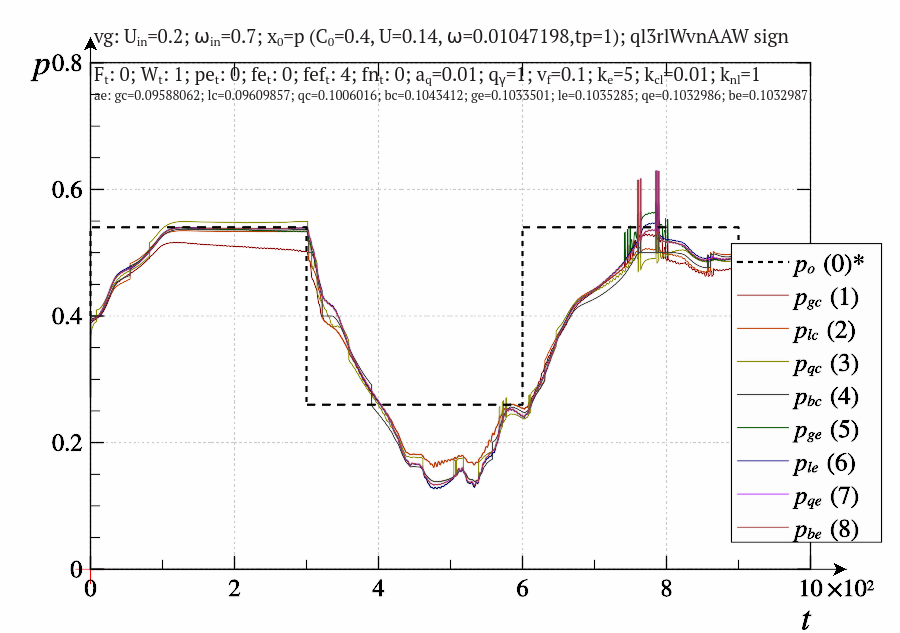
\includegraphics[width=0.49\textwidth]{p/cha/vg/vg_id-p_t_p_ql3rlWvnAAW_sign.png}
\end{center}
  \caption{Динамика агентов и идентифицируемого значения для системы колебательной системы с гистерезисной возвращающей силой при условии (\ref{atu:eq:po_t_sign})}
\label{atu:f:vg_id_sign}
\end{figure}

В рассматриваемых условиях на величину ошибки идентификации
негативно влияют два фактора: примыкающий к нулевой частоте
участок сплошного спектра, а также отсутствие монотонности критерия
в области минимального значения параметра.
Это приводит к значительным ошибкам в процессе идентификации,
при сохранении работоспособности метода.


На рис.~\ref{atu:f:vg_id_sin}
приведены аналогичные зависимости, то при условии~(\ref{atu:eq:po_t_sign}).

\begin{figure}[ht!]
\begin{center}
  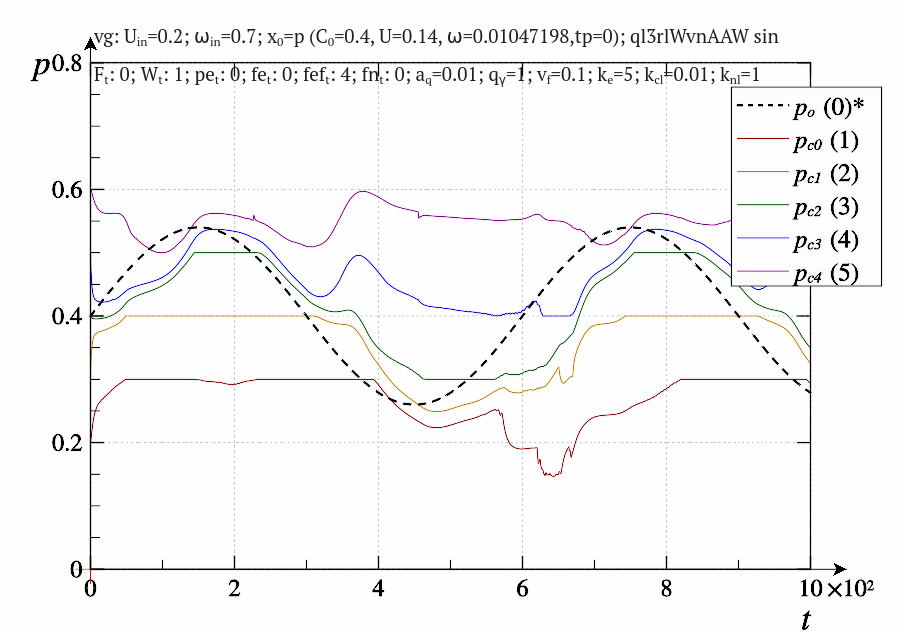
\includegraphics[width=0.49\textwidth]{p/cha/vg/vg_id-p_t_pi_ql3rlWvnAAW_sin.png}
  \hfill
  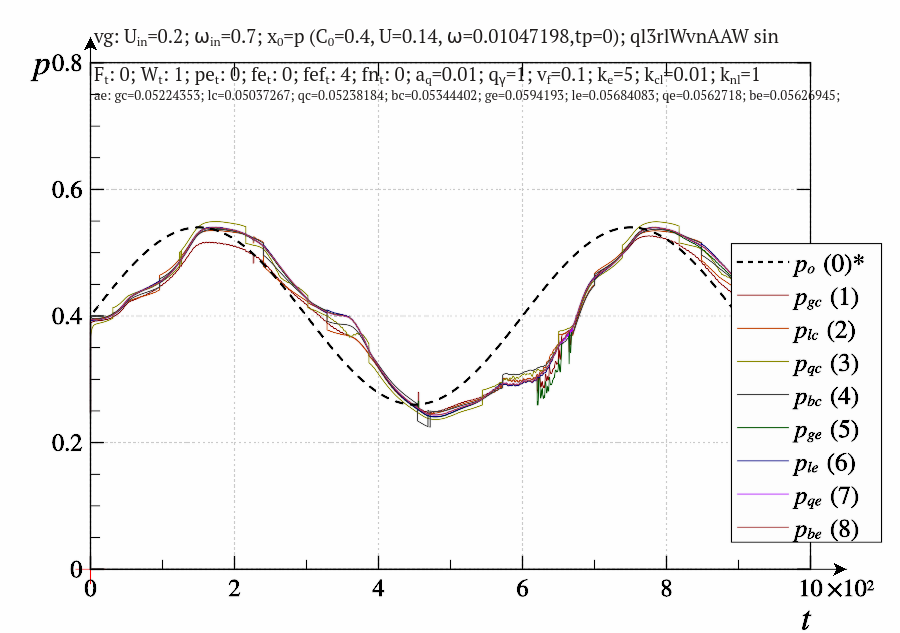
\includegraphics[width=0.49\textwidth]{p/cha/vg/vg_id-p_t_p_ql3rlWvnAAW_sin.png}
\end{center}
  \caption{Динамика агентов и идентифицируемого значения для системы колебательной системы с гистерезисной возвращающей силой при условии (\ref{atu:eq:po_t_sin})}
\label{atu:f:vg_id_sin}
\end{figure}

Более плавное изменение параметра,
как и в предыдущих случаях,
приводит к уменьшению ошибки идентификации.
Однако, вид критерия не позволяет получить
достаточно малую ошибку идентификации.



% }}}2

\subsection{Влияние параметров системы идентификации на ошибку идентификации}  % {{{2

Влияние параметра $a_q$ на ошибку идентификации
для колебательной системы с гистерезисной возвращающей силой
имеет вид, типичный для систем со спектром,
примыкающим к нулевой частоте~(рис.~\ref{atu:f:vg_e_a_q}).
Нет явно выраженного минимума, что свидетельствует
об ограниченности фильтрующих свойств подхода к усреднению критерия.

\begin{figure}[ht!]
\begin{center}
  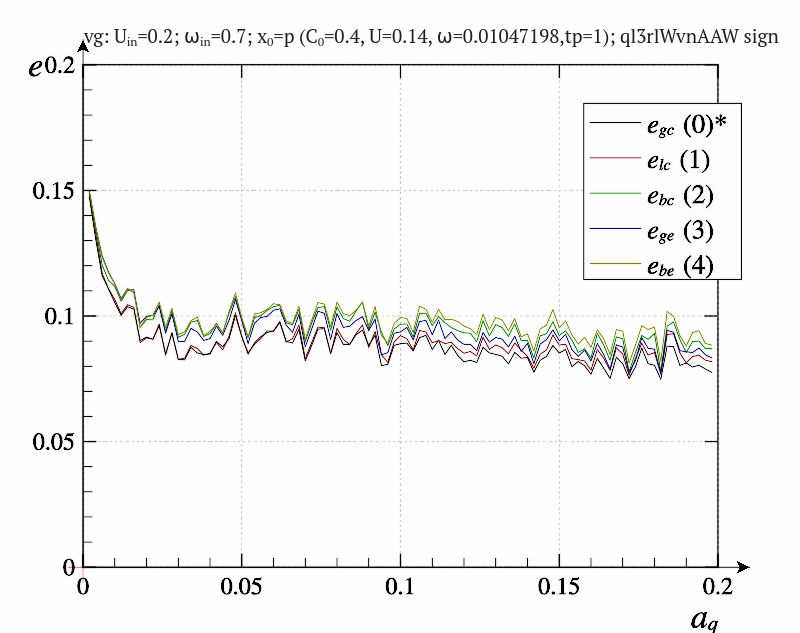
\includegraphics[width=0.49\textwidth]{p/cha/vg/vg_id-p_a_q_sign.png}
  \hfill
  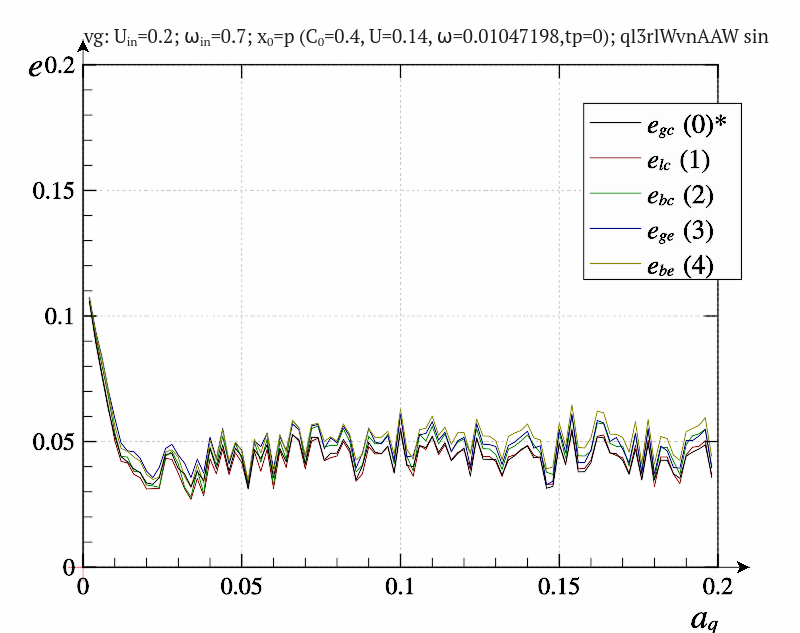
\includegraphics[width=0.49\textwidth]{p/cha/vg/vg_id-p_a_q_sin.png}
\end{center}
  \caption{Зависимости $\bar{e}(a_q)$ для колебательной системы с гистерезисной возвращающей силой}
\label{atu:f:vg_e_a_q}
\end{figure}

На фоне относительно высокой ошибки идентификации,
определяемой свойствами критерия,
зависимость от масштаба функции качества
(рис.~\ref{atu:f:vg_e_q_gamma})
пренебрежимо мала, если, конечно,
параметр $q_\gamma$ системы идентификации
находится в разумных пределах.

\begin{figure}[ht!]
\begin{center}
  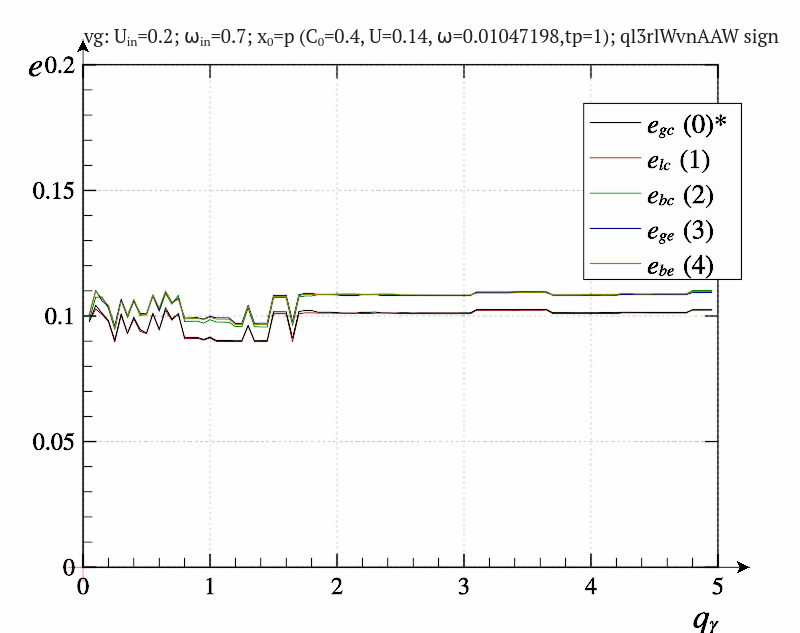
\includegraphics[width=0.49\textwidth]{p/cha/vg/vg_id-p_q_gamma_sign.png}
  \hfill
  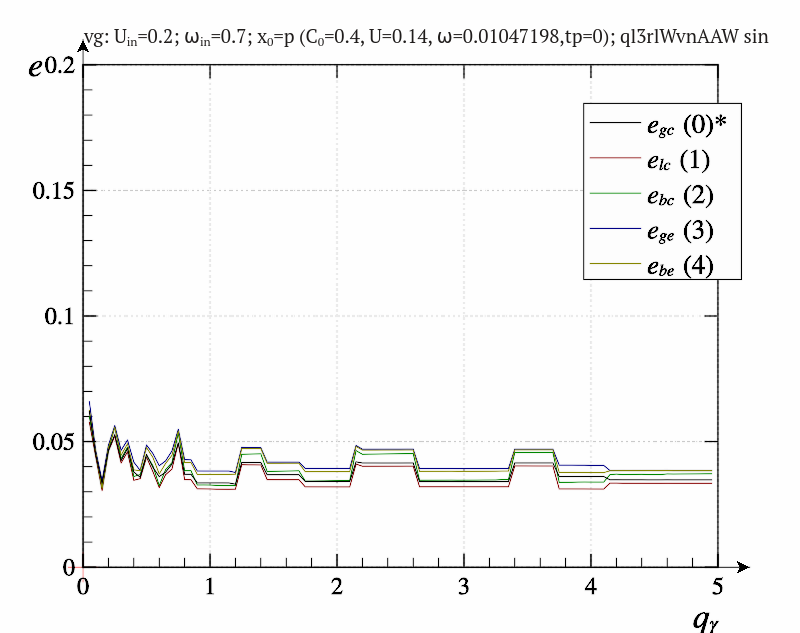
\includegraphics[width=0.49\textwidth]{p/cha/vg/vg_id-p_q_gamma_sin.png}
\end{center}
  \caption{Зависимости $\bar{e}(q_\gamma)$ для колебательной системы с гистерезисной возвращающей силой}
\label{atu:f:vg_e_q_gamma}
\end{figure}

Свойства критерия $q_{rx}$ для данной системы
также обуславливают слабую зависимость ошибки идентификации
от параметра $v_f$ (рис.~\ref{atu:f:vg_e_v_f}).
Для быстро изменяющегося параметра перемещение агентов
может быть не порванным.

\begin{figure}[ht!]
\begin{center}
  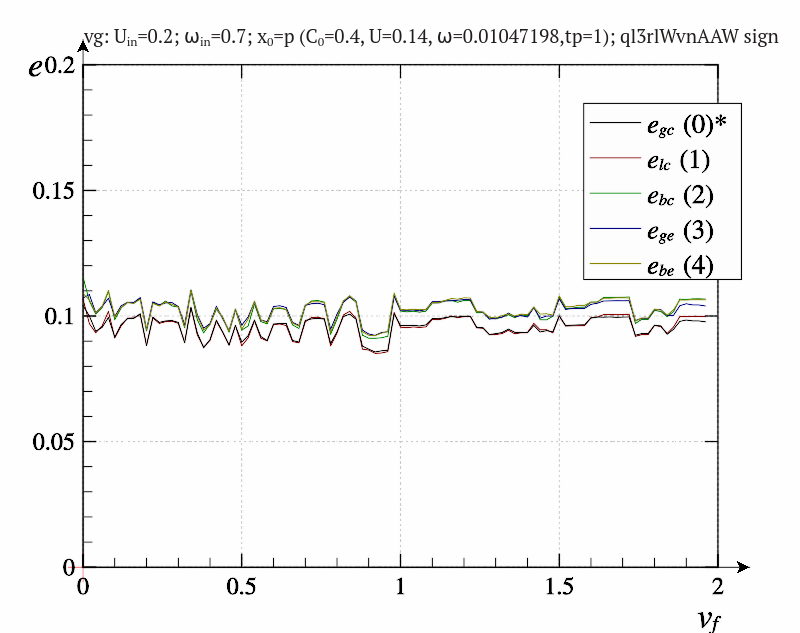
\includegraphics[width=0.49\textwidth]{p/cha/vg/vg_id-p_v_f_sign.png}
  \hfill
  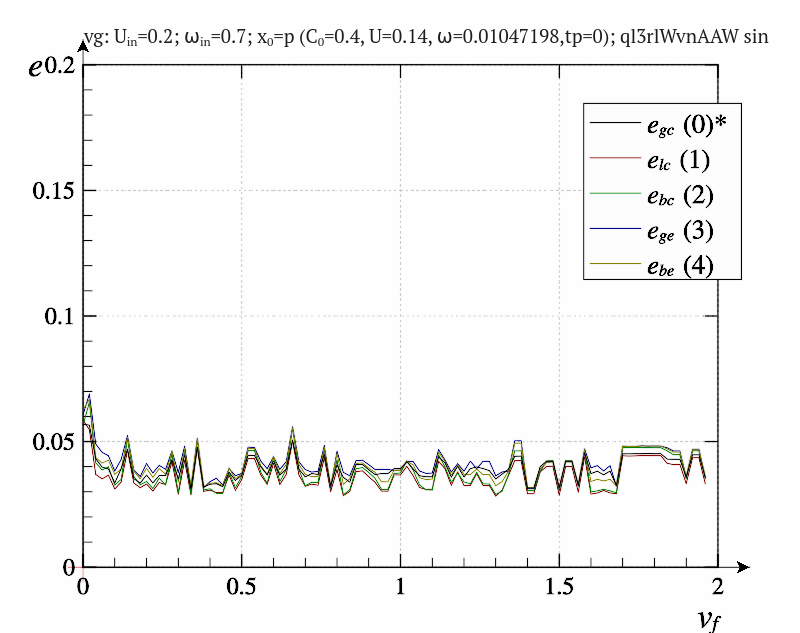
\includegraphics[width=0.49\textwidth]{p/cha/vg/vg_id-p_v_f_sin.png}
\end{center}
  \caption{Зависимости $\bar{e}(v_f)$ для колебательной системы с гистерезисной возвращающей силой}
\label{atu:f:vg_e_v_f}
\end{figure}

Совершенно аналогичная картина наблюдается для параметра $k_e$~(рис.~\ref{atu:f:vg_e_k_e}).

\begin{figure}[ht!]
\begin{center}
  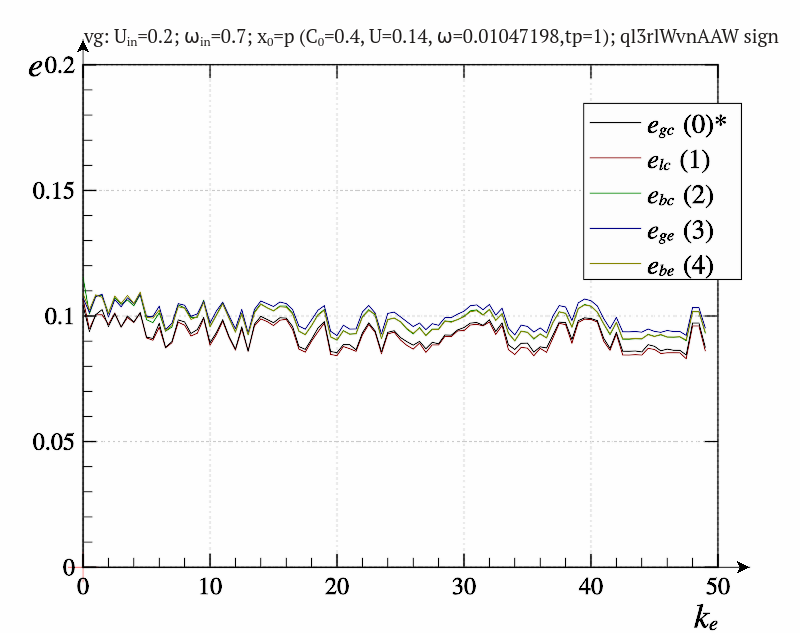
\includegraphics[width=0.49\textwidth]{p/cha/vg/vg_id-p_k_e_sign.png}
  \hfill
  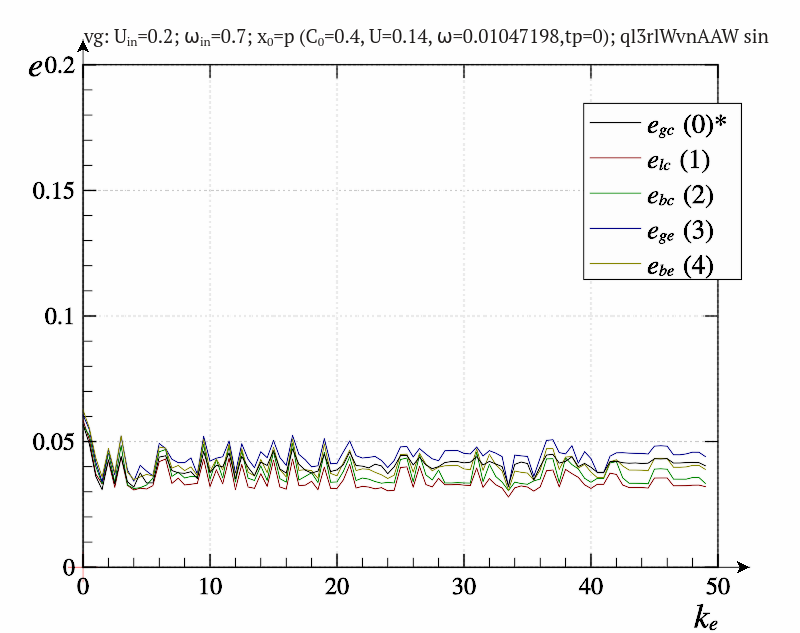
\includegraphics[width=0.49\textwidth]{p/cha/vg/vg_id-p_k_e_sin.png}
\end{center}
  \caption{Зависимости $\bar{e}(k_e)$ для колебательной системы с гистерезисной возвращающей силой}
\label{atu:f:vg_e_k_e}
\end{figure}

Вид зависимости $\bar{e}(k_{nl})$ для рассматриваемой системы имеет определённые
отличия~(рис.~\ref{atu:f:vg_e_k_nl}).
Слабо выраженный, но всё же заметный минимум наблюдается
при значениях $k_{nl}$, практически совпадающих с используемым значением $k_e$.
Это можно объяснить тем, что большее квазиравновесное расстояние
между агентами позволяет в какой-то мере нивелировать
возмущения критерия небольшой амплитуды.

\begin{figure}[ht!]
\begin{center}
  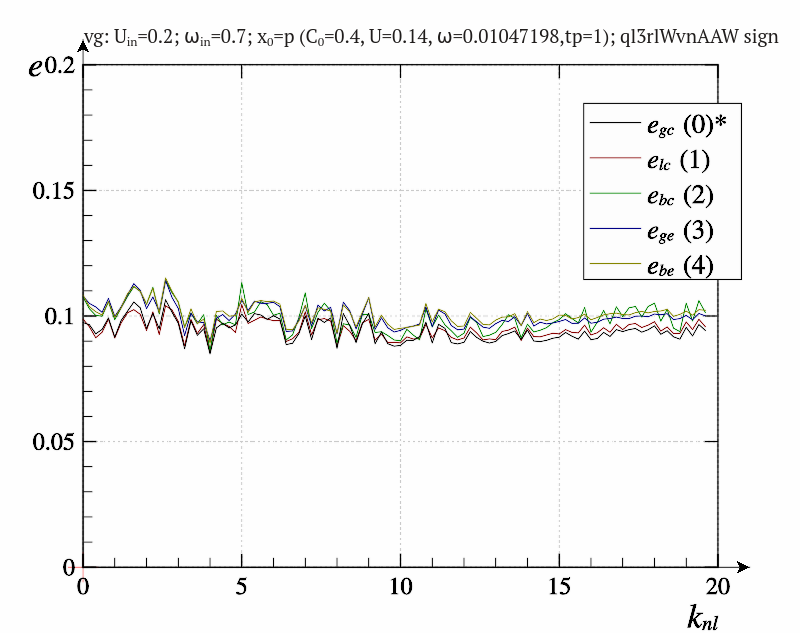
\includegraphics[width=0.49\textwidth]{p/cha/vg/vg_id-p_k_nl_sign.png}
  \hfill
  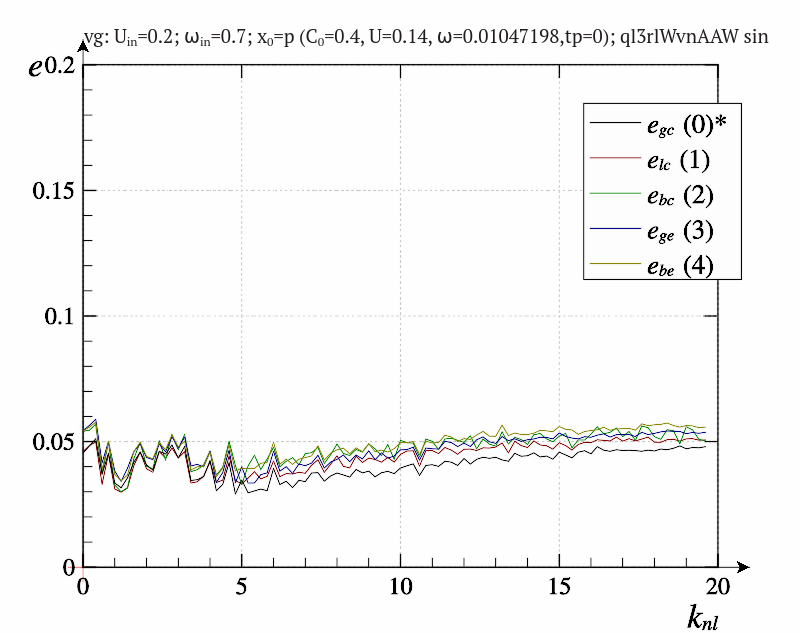
\includegraphics[width=0.49\textwidth]{p/cha/vg/vg_id-p_k_nl_sin.png}
\end{center}
  \caption{Зависимости $\bar{e}(k_{nl})$ для колебательной системы с гистерезисной возвращающей силой}
\label{atu:f:vg_e_k_nl}
\end{figure}

Использование неоднозначного критерия,
в совокупности с ограничениями на перемещения агентов
делает зависимость $\bar{e}(k_{cl})$ (рис.~\ref{atu:f:vdp_e_k_cl})
практически не наблюдаемой.


\begin{figure}[ht!]
\begin{center}
  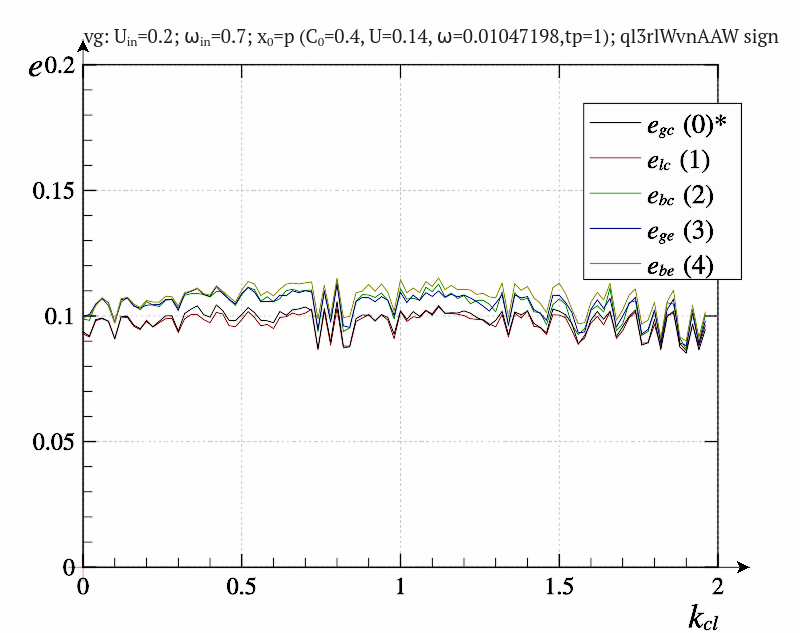
\includegraphics[width=0.49\textwidth]{p/cha/vg/vg_id-p_k_cl_sign.png}
  \hfill
  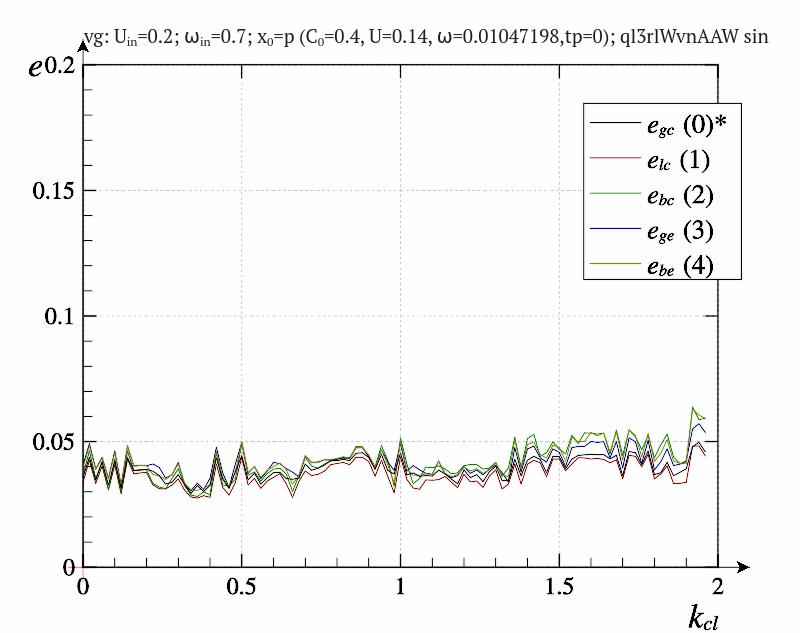
\includegraphics[width=0.49\textwidth]{p/cha/vg/vg_id-p_k_cl_sin.png}
\end{center}
  \caption{Зависимости $\bar{e}(k_{cl})$ для колебательной системы с гистерезисной возвращающей силой}
\label{atu:f:vg_e_k_cl}
\end{figure}



% }}}2


\subsection{Выводы}  % {{{2

Результаты моделирования
как динамики системы~(\ref{atu:eq:vglass})
так и процессов идентификации её параметра $x_0$
позволяют в сделать следующие выводы:

\begin{itemize}

  \item
    Колебательная система с гистерезисной возвращающей силой
    под воздействием внешней гармонического возмущения
    может демонстрировать различные виды динамик, в
    том числе сложно-периодическую и хаотическую.


  \item
    Критерий $q_{rx}$ хоть и подходит для идентификации параметра ``$x_0$''
    колебательной системы с гистерезисной возвращающей силой,
    но обладает нарушениями монотонности,
    что существенно увеличивает ошибку идентификации.

  \item
    Наличие сплошного спектра системы, примыкающего к нулевой частоте,
    усложняет задачу корректного усреднения критерия.

  \item
    Группа методов ql3rlWvnAAW показала свою хорошую работоспособность
    даже в условиях использования критерия с ограниченной применимостью.


\end{itemize}
% }}}2

% }}}1

% vim: fdm=marker foldlevel=1 foldignore="%#" fdc=4 ft=tex
